%% ============================================================
%%  FIGNN - IEEE Access submission
%%  Complete manuscript update - authoritative values from
%%  loso_all29_subject_metrics.csv, stage2_calibration_comparison_64D.csv,
%%  stage2_calibration_comparison_64D_paired_tests.csv
%%  and train.py / model.py (subject-wise split, lowest val SupCon loss)
%% ============================================================
\let\TeXyear\year
\documentclass{ieeeaccess}
\let\setyear\year
\let\year\TeXyear

\usepackage{cite}
\usepackage{amsmath,amssymb,amsfonts}
\usepackage{algorithmic}
\usepackage{graphicx}
\usepackage{textcomp}
\usepackage{booktabs}
\usepackage{multirow}
\usepackage{array}

\begin{document}

\title{Frequency-Informed Graph Neural Network for Cross-Subject EEG
       Workload Representation and Personal Calibration}

\author{
\uppercase{Vignesh Jaisankar}\authorrefmark{1},
\uppercase{Dr. Shridevi S }\authorrefmark{1},
\uppercase{Dr. Harish}\authorrefmark{1}
}

\address[1]{Centre for Neuroinformatics, Vellore Institute of Technology,
            Chennai, India}

\markboth
{Vignesh Jaisankar: FIGNN for EEG Workload Representation and Personal Calibration}
{Vignesh Jaisankar: FIGNN for EEG Workload Representation and Personal Calibration}

\begin{abstract}
Electroencephalographic (EEG) representations of cognitive workload
exhibit substantial inter-subject variability, and population-level models
rarely transfer directly to unseen individuals without adaptation. This paper
proposes a Frequency-Informed Graph Neural Network (FIGNN) that encodes EEG
epochs into a normalized 64-dimensional latent space by combining relative
frequency-band power at electrode nodes with frequency-specific phase-locking
value (PLV) connectivity at graph edges. A learnable four-band
frequency-weighting layer modulates edge attributes before two edge-aware
graph-attention layers produce the graph-level embedding, trained using
supervised contrastive learning. The frequency-weighting layer assigns the
largest learned coefficients to beta ($w=0.364$) and alpha ($w=0.291$).

Transferability is evaluated under strict 29-fold leave-one-subject-out
(LOSO) cross-validation on the COG-BCI dataset. The primary criterion is
the segment-membership test: 23 of 29 held-out subjects (79.31\%; exact
binomial 95\% CI: 60.3--92.0\%; one-sided $p=0.0012$ vs.\ chance $p=0.5$)
satisfy $0\leq\rho_s\leq1$, meaning that the 1-back latent centroid projects
onto the 0-back-to-2-back segment. The supporting distance-ordering criterion
$d_{01}<d_{02}$ holds for 27 of 29 subjects. Mean alignment-free trajectory
metrics are: path efficiency $0.819\pm0.170$, $d_{01}/d_{02}$
$0.477\pm0.270$, trajectory angle $73.2\pm39.7^{\circ}$, and relative 1-back
position $0.271\pm0.291$. As a secondary descriptive shape-correspondence
measure, the mean Procrustes similarity is $0.878\pm0.155$.

A second-stage frozen-encoder geometric calibration experiment evaluates
whether the transferred geometry can be personalized without retraining.
Four methods are compared: population-only ($\bar{\epsilon}=0.0649$),
midpoint ($0.0522$), regression ($0.0511$), and frozen geometric calibration
($0.0345$). The frozen geometric method reduces mean 64-dimensional estimation
error by 46.74\% relative to the population-only baseline and improves 22
of 29 subjects; a paired Wilcoxon signed-rank test gives $W=377$,
Holm-corrected $p=0.000404$, Cohen's $d_z=0.821$. These results, obtained
on COG-BCI, support a population-to-personalization framework in which a
common latent workload geometry is transferred to an unseen subject and
subsequently adapted using resting-state and known 2-back anchors, without
any encoder retraining.
\end{abstract}

\begin{keywords}
EEG, cognitive workload, graph neural network, phase-locking value,
supervised contrastive learning, cross-subject representation,
geometric calibration, latent representation
\end{keywords}

\titlepgskip=-15pt
\makeatletter
\gdef\thevol{14}
\gdef\theyear{2026}
\makeatother
\maketitle

%% ============================================================
\section{Introduction}
\label{sec:intro}
%% ============================================================

Electroencephalography (EEG) provides a non-invasive, temporally precise
measure of neural activity and is extensively studied for cognitive workload
estimation. Workload-related EEG dynamics are commonly characterized through
spectral measures in the delta, theta, alpha, and beta frequency bands, yet
the same cognitive condition can occupy substantially different regions of
feature space across individuals \cite{chikhi2022}. This inter-subject
variability poses a fundamental challenge: population-level representations
trained on many subjects may not transfer reliably to an unseen individual
without some form of adaptation.

A predominant approach formulates workload estimation as multi-class
classification \cite{cao2022,wei2025}. While classification is useful for
distinguishing predefined workload levels, it does not reveal whether a
learned representation preserves the \emph{relative structure} of workload
states for a subject excluded from training. For graded paradigms such as
N-back, where task demand increases monotonically, conditions can instead be
viewed as an ordered trajectory in latent space. Evaluating representation
transfer through latent geometry provides a more principled test of
structural transferability than classification accuracy alone.

Graph neural networks (GNNs) offer a principled framework for multichannel
EEG because electrodes correspond naturally to graph nodes and functional
relationships between electrodes to graph edges \cite{klepl2024}. Frequency
information can be incorporated at the node level as band-power features and
at the connectivity level as phase-synchronization measures. Learnable
frequency-weighting mechanisms that adapt spectral emphasis to the task have
also emerged as an effective design choice for EEG decoding \cite{ding2025freq}.

This paper introduces a Frequency-Informed Graph Neural Network (FIGNN) that
combines relative four-band power at electrode nodes with frequency-specific
PLV connectivity at graph edges. A learnable band-weighting layer modulates
edge attributes before two edge-aware graph-attention layers produce a
normalized 64-dimensional embedding. Supervised contrastive learning
organizes the latent space by workload condition; the observed workload
trajectory ordering is an emergent geometric property of the learned
representation, not an ordering explicitly imposed by the contrastive objective.

Stage~1 asks whether the resulting workload geometry transfers to subjects
completely excluded from training, using a strict 29-fold LOSO protocol.
The primary transferability criterion is a segment-membership test based on
the scalar projection of the unseen subject's 1-back centroid onto the
population 0-back-to-2-back direction. Stage~2 then asks whether the
transferred geometry can be personalized using only resting-state and known
2-back latent anchors, without updating any encoder parameters.

The contributions are:
\begin{enumerate}
  \item a frequency-informed EEG graph representation that combines relative
        four-band power node features, band-specific PLV edge attributes, and
        a learnable four-band frequency-weighting layer within an edge-aware
        graph-attention encoder;
  \item a strict 29-subject LOSO evaluation of cross-subject workload
        trajectory transfer, with the primary segment-membership criterion
        satisfied by 23/29 subjects (79.31\%, $p=0.0012$), a supporting
        distance-ordering criterion at 27/29, and mean Procrustes similarity
        $0.878\pm0.155$ as a secondary descriptive measure; and
  \item a frozen-encoder geometric calibration procedure that uses resting-state
        and known 2-back anchors to estimate an unseen 1-back centroid, reducing
        mean 64-dimensional error from 0.0649 to 0.0345 (46.74\%,
        Holm-corrected $p=0.000404$) without any encoder retraining.
\end{enumerate}

%% ============================================================
\section{Related Work}
\label{sec:related}
%% ============================================================

\subsection{Graph Neural Networks for EEG}

GNNs have emerged as a natural framework for multichannel EEG analysis because
they represent electrode relationships through a graph topology that reflects
underlying neural geometry. A comprehensive survey identifies graph construction
strategy, node feature design, and graph propagation mechanism as the principal
design axes of GNN-based EEG systems \cite{klepl2024}. Within the cognitive
workload domain, Cao~\emph{et al.} exploited functional brain connectivity for
multi-level workload classification \cite{cao2022}. Wei~\emph{et al.} combined
frequency-domain features with multiple connectivity measures in a stacked
graph-attention architecture (SGATCN) for task-independent workload
discrimination, representing the most closely related prior work \cite{wei2025}.
FIGNN differentiates itself from SGATCN by (i)~introducing a learnable
frequency-weighting mechanism directly on graph edge attributes and
(ii)~evaluating representation transfer through latent trajectory geometry
rather than classification accuracy.

\subsection{Frequency-Domain Features and Learnable Band Weighting}

Spectral decomposition is central to workload analysis because workload-related
neural changes span multiple frequency bands \cite{chikhi2022}. Fixed band-power
features treat all bands equally. Recent EEG decoding work has addressed this
limitation through learnable frequency-weighting mechanisms \cite{ding2025freq}.
FIGNN applies the weighting operation directly to frequency-specific edge
attributes, enabling the model to modulate connectivity information
independently of node features before graph attention.

\subsection{Phase-Locking Value Connectivity}

Phase-locking value (PLV) quantifies the consistency of instantaneous phase
differences between two signals and is a frequency-specific measure of
functional synchronization widely applied in EEG analysis
\cite{lachaux1999}. FIGNN retains PLV as the connectivity representation
across all four canonical bands as separate edge features. Edge-aware graph
attention allows these connectivity attributes to modulate message-passing
computations \cite{velickovic2018}.

\subsection{Subject Adaptation and Resting-State Anchors}

Cross-subject generalization and subject-specific adaptation are longstanding
challenges in EEG-based brain-computer interfaces. Resting-state EEG has been
explored as a low-cost source of subject-specific information for adapting
models to unseen individuals \cite{an2024}. Individual EEG measures exhibit
meaningful longitudinal stability \cite{uudeberg2025}, supporting the use of
a small number of subject-specific measurements to anchor a pre-trained
representation. The Stage~2 procedure keeps the FIGNN encoder entirely frozen
and uses latent anchors to adjust the position of the workload trajectory
geometrically, without any gradient-based adaptation.

%% ============================================================
\section{Methodology}
\label{sec:method}
%% ============================================================

\subsection{Framework Overview}

The proposed framework is organized into two sequential stages, illustrated
in Fig.~\ref{fig:pipeline}. Stage~1 trains a population representation under
strict LOSO evaluation and assesses whether the resulting workload geometry
transfers to subjects excluded from training. Stage~2 keeps the fold-specific
FIGNN encoder frozen and uses subject-specific anchor states to personalize
the placed workload trajectory without updating any model parameters.

\begin{figure}[!t]
\centering
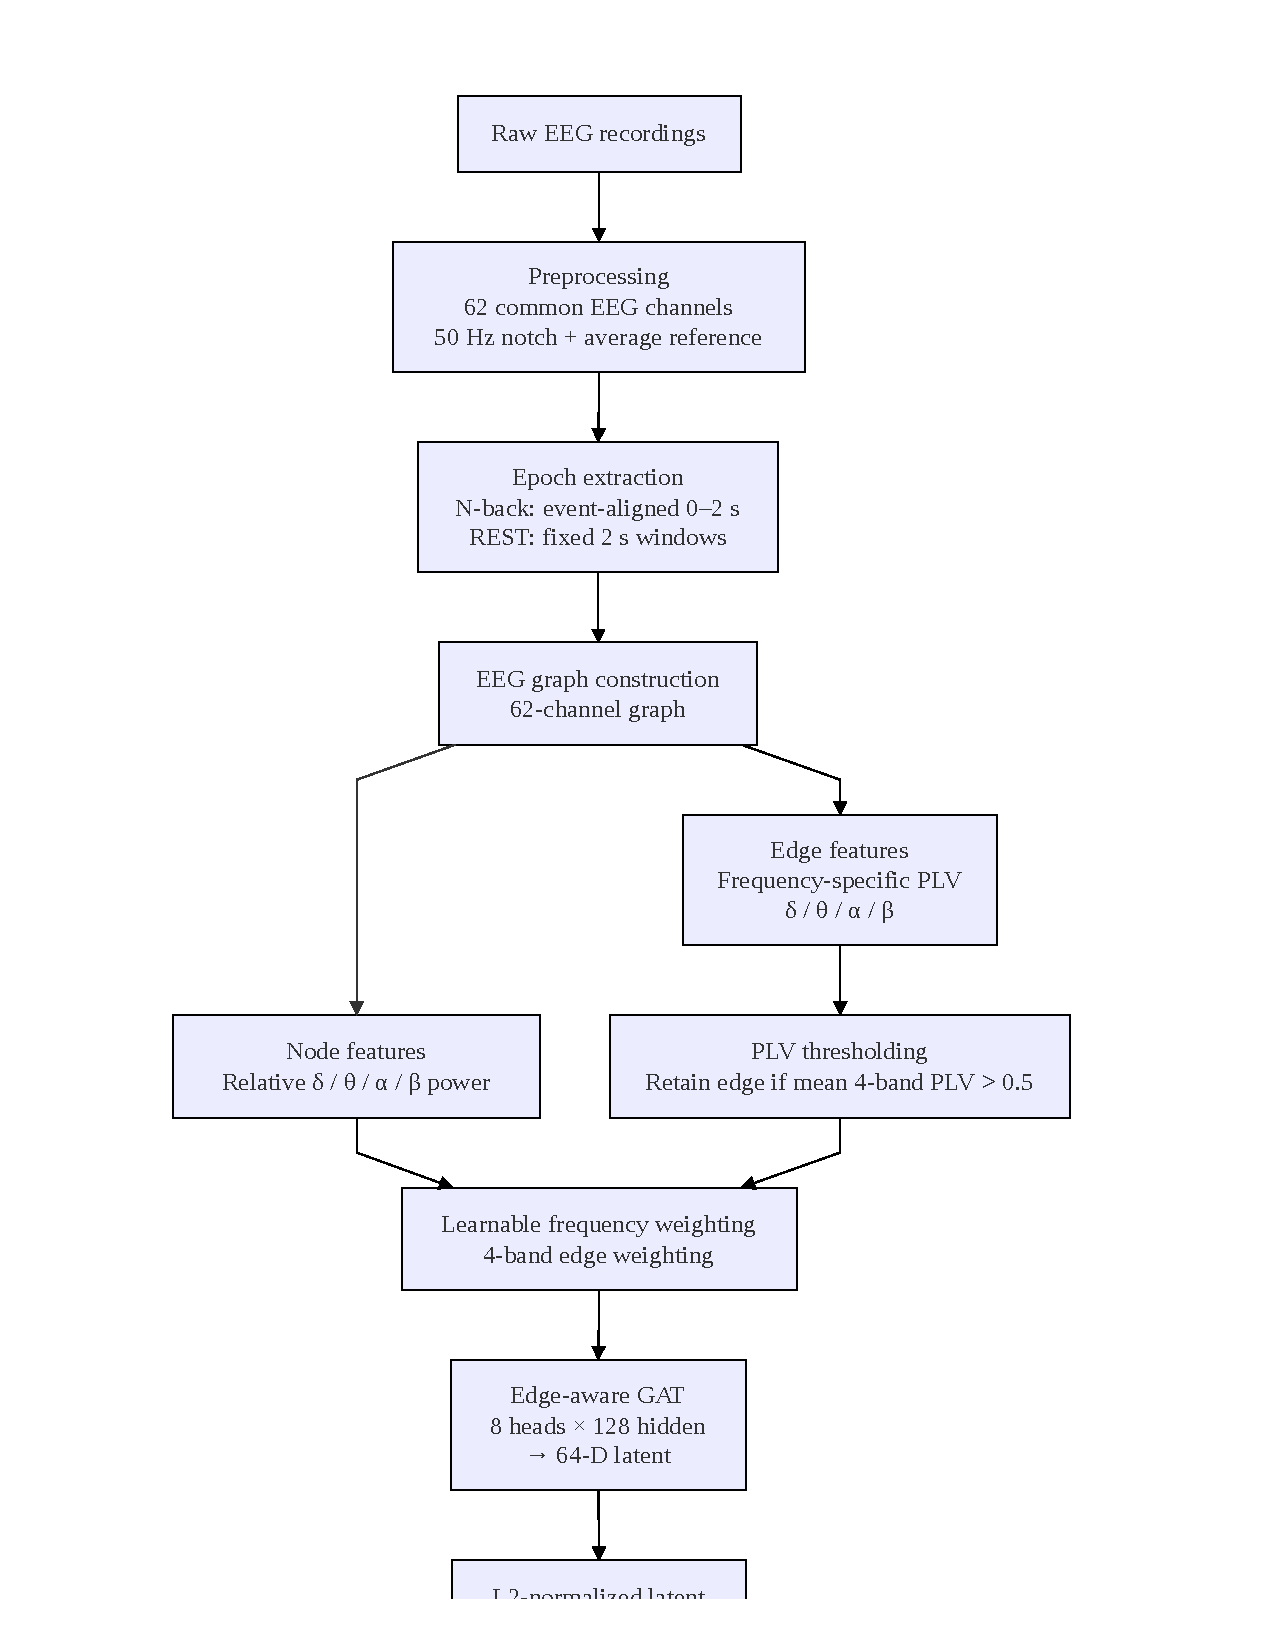
\includegraphics[width=\columnwidth]{figures/FIGNN_stage1_drawio.pdf}
\caption{Overall FIGNN framework. Event-aligned EEG epochs are converted into
62-channel graphs with relative four-band power at the nodes and
frequency-specific PLV at the edges. A learnable frequency-weighting layer
modulates edge attributes before two edge-aware graph-attention layers produce
a normalized 64-dimensional embedding trained with supervised contrastive
learning. Stage~1 evaluates cross-subject representation transfer under strict
29-fold LOSO; Stage~2 applies frozen-encoder geometric calibration.}
\label{fig:pipeline}
\end{figure}

\subsection{EEG Graph Representation}

Each preprocessed EEG epoch is represented as a graph
\begin{equation}
  G = (V, E, X, E_f),
\end{equation}
where $V$ denotes the set of EEG electrodes, $E$ the retained
functional-connectivity edges, $X$ the node feature matrix, and $E_f$ the
frequency-specific edge attribute matrix. The final graph uses 62 common EEG
channels.

\subsubsection{Node Features}
For channel $i$, the node feature vector encodes relative band power:
\begin{equation}
  \mathbf{x}_i =
  [P_i^{\delta},\; P_i^{\theta},\; P_i^{\alpha},\; P_i^{\beta}],
\end{equation}
where the relative power in band $b$ is
\begin{equation}
  P_i^b =
  \frac{P_{i,\mathrm{abs}}^b}
       {\displaystyle\sum_{k\in\{\delta,\theta,\alpha,\beta\}}
        P_{i,\mathrm{abs}}^k}.
\end{equation}

\subsubsection{Edge Features and Connectivity Threshold}
Phase-locking value is computed within each band:
\begin{equation}
  \mathrm{PLV}_{ij}^{b}
  = \left|\frac{1}{T}\sum_{t=1}^{T}
    e^{\,j(\phi_i^b(t)-\phi_j^b(t))}\right|.
\end{equation}
The four per-band values form the edge attribute vector
\begin{equation}
  \mathbf{e}_{ij}
  = [\mathrm{PLV}_{ij}^{\delta},\;
     \mathrm{PLV}_{ij}^{\theta},\;
     \mathrm{PLV}_{ij}^{\alpha},\;
     \mathrm{PLV}_{ij}^{\beta}].
\end{equation}
An undirected edge is retained when the mean four-band PLV exceeds 0.5.
Each retained edge is added in both directions for bidirectional message
passing.

\subsection{EEG Preprocessing}

EEGLAB recordings are loaded via MNE-Python. Channels outside the common
62-channel set are removed. A 50-Hz notch filter removes power-line
interference, and average reference re-referencing is applied. Signals are
separately band-pass filtered into delta (1--4~Hz), theta (4--8~Hz), alpha
(8--13~Hz), and beta (13--30~Hz).

For N-back recordings, stimulus annotations are used to extract event-aligned
epochs spanning 0--2~s from stimulus onset. This window is intentionally
aligned to the post-stimulus interval across all trials; it is not arbitrary
graph chunking. Resting-state recordings are segmented into non-overlapping
2-s windows. We acknowledge that the lower end of the delta band (1--4~Hz)
yields a limited number of cycles within a 2-s epoch; this is a methodological
limitation noted in Section~\ref{sec:discussion}. Resting-state epochs are
retained separately for Stage~2 anchor computation and excluded from
Stage~1 training.

The resulting graph representations are
\begin{equation}
  X \in \mathbb{R}^{62 \times 4}, \qquad
  E_f \in \mathbb{R}^{N_e \times 4},
\end{equation}
where $N_e$ is the number of retained edges.

\subsubsection{Node Feature Normalization}
The four relative band-power node features are z-score normalized. Within
each LOSO fold, the mean and standard deviation are computed exclusively from
the fold's training subjects' graphs and applied unchanged to training,
validation, and held-out test graphs. No log transform is applied, and this
normalization does not affect PLV edge attributes or L2-normalized latent
embeddings.

\subsection{Frequency-Informed Graph Neural Network}

The FIGNN encoder consists of a learnable frequency-weighting layer followed
by two edge-aware graph-attention (GAT) layers.

\subsubsection{Learnable Frequency Weighting}
Let $\boldsymbol{\theta} \in \mathbb{R}^{4}$ denote four learnable scalar
parameters, one per frequency band. The normalized weights are
\begin{equation}
  \mathbf{w} = \operatorname{softmax}(\boldsymbol{\theta}),
\end{equation}
and edge attributes are modulated element-wise:
\begin{equation}
  \mathbf{e}'_{ij} = \mathbf{e}_{ij} \odot \mathbf{w}.
\end{equation}

\subsubsection{Graph-Attention Layers}
The first edge-aware GAT layer operates on four-dimensional node features with
eight attention heads and 128 output dimensions per head. Concatenation yields
a 1\,024-dimensional intermediate node representation, which is a direct
consequence of $8 \times 128$ concatenation rather than an additional
fully-connected expansion. Layer normalization, ELU activation, and dropout
($p=0.3$) follow. The second edge-aware GAT layer maps the 1\,024-dimensional
representations to 64 dimensions using a single attention head. Layer
normalization and global mean pooling produce
\begin{equation}
  \mathbf{h}_G = \operatorname{MeanPool}\!\left(\mathbf{H}^{(2)}\right).
\end{equation}
The embedding is L2-normalized:
\begin{equation}
  \mathbf{z}
  = \frac{\mathbf{h}_G}{\|\mathbf{h}_G\|_2},
  \qquad
  \mathbf{z} \in \mathbb{R}^{64}.
\end{equation}
The total trainable parameter count is approximately 80.5k.

\subsection{Supervised Contrastive Representation Learning}

FIGNN is trained using supervised contrastive learning \cite{khosla2020}.
For a batch of $N$ embeddings, samples sharing the same workload label form
positive pairs; samples with different labels provide negative comparisons.
For anchor sample $i$:
\begin{equation}
  P(i) = \{p : p \neq i,\; y_p = y_i\}, \quad
  A(i) = \{a : a \neq i\}.
\end{equation}
The loss is
\begin{equation}
  \mathcal{L}
  = -\sum_i
    \frac{1}{|P(i)|}
    \sum_{p \in P(i)}
    \log
    \frac{
      \exp(\mathbf{z}_i^{\top}\mathbf{z}_p / \tau)
    }{
      \displaystyle\sum_{a \in A(i)}
      \exp(\mathbf{z}_i^{\top}\mathbf{z}_a / \tau)
    },
  \label{eq:supcon}
\end{equation}
with $\tau = 0.1$. This objective pulls embeddings of the same workload label
together and separates embeddings of different labels; it does not explicitly
impose an ordinal constraint on the 0-back, 1-back, 2-back sequence. The
observed workload trajectory ordering is an emergent geometric property of the
learned representation, not an ordering explicitly enforced by the loss
function.

\subsection{Training Configuration}

\begin{table}[!t]
  \caption{FIGNN Training Hyperparameters}
  \label{tab:hyperparams}
  \centering
  \begin{tabular}{lc}
    \toprule
    \textbf{Hyperparameter} & \textbf{Value} \\
    \midrule
    Optimizer              & AdamW \\
    Learning rate          & $1\times10^{-3}$ \\
    Weight decay           & $1\times10^{-4}$ \\
    LR schedule            & Cosine annealing (min $1\times10^{-5}$) \\
    Epochs                 & 500 \\
    Batch size             & 128 \\
    Dropout                & 0.3 \\
    Contrastive $\tau$     & 0.1 \\
    Latent dimension       & 64 \\
    GAT layer 1            & 8 heads, 128 hidden \\
    GAT layer 2            & 1 head, 64-D \\
    Trainable parameters   & ${\approx}80.5$k \\
    \bottomrule
  \end{tabular}
\end{table}

Table~\ref{tab:hyperparams} summarizes the training configuration. A
class-balanced weighted random sampler is used at each iteration. Within each
LOSO fold, the 28 training subjects are partitioned into training and validation
subjects using a fixed seeded subject-wise 85/15 split; no subject contributes
graphs to both partitions. The fold-specific normalization statistics are
computed from training-partition graphs only and applied to training,
validation, and held-out test graphs. The checkpoint achieving the lowest
validation SupCon loss is retained as the fold-specific model. The held-out
LOSO subject is excluded entirely from training and checkpoint selection.

%% ============================================================
\section{Stage 1: Cross-Subject Representation Transfer}
\label{sec:stage1}
%% ============================================================

\subsection{Strict Leave-One-Subject-Out Protocol}

Stage~1 applies a 29-fold LOSO protocol. For fold $s$,
\begin{equation}
  \mathcal{D}_{\mathrm{train}}^{(s)}
  = \mathcal{D} \setminus \mathcal{D}_s.
\end{equation}
All epochs from subject $s$ are excluded from training, validation, and
checkpoint selection. Resting-state graphs are excluded from Stage~1 training;
the three N-back conditions define the ordered workload sequence
$0\text{-back}\rightarrow1\text{-back}\rightarrow2\text{-back}$.

For workload condition $c$ and held-out subject $s$, the latent centroid is
\begin{equation}
  \mathbf{C}_{s,c}
  = \frac{1}{N_{s,c}}\sum_{i=1}^{N_{s,c}} \mathbf{z}_{s,c,i}.
\end{equation}
The population centroid averages over the 28 training-subject centroids.

\subsection{Latent Workload Trajectory Geometry}

The subject workload trajectory is the ordered triplet
\begin{equation}
  T_s = [\mathbf{C}_{s,0},\; \mathbf{C}_{s,1},\; \mathbf{C}_{s,2}].
\end{equation}
Pairwise centroid distances are
\begin{align}
  d_{01} &= \|\mathbf{C}_{s,0} - \mathbf{C}_{s,1}\|_2, \label{eq:d01}\\
  d_{02} &= \|\mathbf{C}_{s,0} - \mathbf{C}_{s,2}\|_2, \label{eq:d02}\\
  d_{12} &= \|\mathbf{C}_{s,1} - \mathbf{C}_{s,2}\|_2. \label{eq:d12}
\end{align}

\subsubsection{Primary Criterion: Segment Membership}
The primary transferability criterion tests whether the held-out subject's
1-back centroid projects onto the 0-back-to-2-back segment. The scalar
projection coefficient is
\begin{equation}
  \rho_s =
  \frac{(\mathbf{C}_{s,1} - \mathbf{C}_{s,0})^{\top}
        (\mathbf{C}_{s,2} - \mathbf{C}_{s,0})}
       {\|\mathbf{C}_{s,2} - \mathbf{C}_{s,0}\|_2^2}.
  \label{eq:rho}
\end{equation}
The primary criterion $0 \leq \rho_s \leq 1$ holds when the projected 1-back
centroid lies \emph{on} the 0-back-to-2-back segment, establishing that
1-back is geometrically intermediate between the two extreme workload states.
The perpendicular deviation from the segment is
\begin{equation}
  \delta_s =
  \bigl\|\mathbf{C}_{s,1}
  - \bigl[\mathbf{C}_{s,0}
    + \rho_s(\mathbf{C}_{s,2} - \mathbf{C}_{s,0})\bigr]\bigr\|_2.
\end{equation}

\subsubsection{Supporting Criterion: Distance Ordering}
The condition $d_{01} < d_{02}$ is a weaker supporting criterion: it indicates
that 1-back is closer to 0-back than 2-back is, but does not establish
that 1-back lies between them on the segment. Both criteria are reported;
only segment membership is used as primary evidence.

\subsubsection{Additional Alignment-Free Diagnostics}
Three scalar quantities characterize the trajectory shape without requiring
alignment to the population template. The relative step sizes are
\begin{equation}
  \rho_{02} = \frac{d_{01}}{d_{02}}, \qquad
  \rho_{12} = \frac{d_{12}}{d_{02}}.
\end{equation}
The interior trajectory angle at the 1-back centroid is
\begin{equation}
  \psi_s = \arccos\!\left(
  \frac{(\mathbf{C}_{s,0}-\mathbf{C}_{s,1})^{\top}(\mathbf{C}_{s,2}-\mathbf{C}_{s,1})}
       {d_{01}\,d_{12}}\right).
  \label{eq:angle}
\end{equation}
Path efficiency compares the direct 0-back-to-2-back displacement with the
two-step path length:
\begin{equation}
  \eta_s = \frac{d_{02}}{d_{01} + d_{12}}.
  \label{eq:efficiency}
\end{equation}
These quantities are computed in the original 64-dimensional latent space
and do not require alignment.

\subsubsection{Secondary Descriptive Measure: Procrustes Similarity}
Trajectory shape correspondence with the population template is additionally
quantified using Procrustes analysis \cite{gower1975}. Population and subject
centroid matrices are aligned to remove translation, scale, and rotation.
Let $D_s$ denote the Procrustes disparity; trajectory similarity is
\begin{equation}
  S_{\mathrm{proc},s} = 1 - D_s.
  \label{eq:procrustes}
\end{equation}
Because this metric is based on only three centroids in a 64-dimensional
space, it is reported as a secondary descriptive complement to the
alignment-free metrics, not as primary transferability evidence.

To characterize subject-level variability, per-subject 95\% bootstrap
confidence intervals for $S_{\mathrm{proc},s}$ were obtained using 1\,000
resamples of each subject's epoch embeddings (median CI width $\approx0.218$).
To assess whether the observed similarities could arise under label permutation,
a Monte Carlo null analysis was conducted: for each subject, 1\,000 random
workload-label assignments were drawn and $S_{\mathrm{proc},s}$ was recomputed
under each assignment. Because only three labels exist, there are only six
unique permutations, so the 1\,000 draws are a Monte Carlo approximation of
this discrete null. The observed similarities are then reported as empirical
percentiles within this null distribution.

\subsubsection{Supporting Orientation Diagnostic: Direction Cosine}
The 0-back-to-2-back direction vectors are
\begin{equation}
  \Delta_s = \mathbf{C}_{s,2} - \mathbf{C}_{s,0}, \qquad
  \widehat{\Delta}_s = \mathbf{C}_{\mathrm{pop},2} - \mathbf{C}_{\mathrm{pop},0},
\end{equation}
with cosine similarity
\begin{equation}
  \cos\theta_s
  = \frac{\Delta_s^{\top}\widehat{\Delta}_s}
         {\|\Delta_s\|_2 \|\widehat{\Delta}_s\|_2}.
\end{equation}
This orientation diagnostic characterizes gross trajectory alignment and is
not treated as evidence independent of Procrustes analysis.

%% ============================================================
\section{Stage 2: Frozen-Encoder Geometric Calibration}
\label{sec:stage2}
%% ============================================================

Stage~2 evaluates whether the transferred workload geometry can be
personalized without updating any FIGNN parameters. For each held-out
subject, the fold-specific encoder and normalization statistics remain frozen.
Four calibration methods are compared, illustrated in
Fig.~\ref{fig:stage2_pipeline}.

\subsection{Calibration Methods}

\subsubsection{Population-Only Baseline}
The population-only baseline uses the mean 1-back centroid of the 28 training
subjects:
\begin{equation}
  \mathbf{C}_{\mathrm{pop},1}
  = \frac{1}{28} \sum_{r \neq s} \mathbf{C}_{r,1}.
\end{equation}
No subject-specific information is used.

\subsubsection{Midpoint}
The midpoint method places the 1-back estimate midway along the subject's
REST-to-2-back direction:
\begin{equation}
  \widehat{\mathbf{C}}_{s,1}^{\mathrm{mid}}
  = \mathbf{R}_s + 0.5\,(\mathbf{C}_{s,2} - \mathbf{R}_s),
\end{equation}
where $\mathbf{R}_s$ is the subject's resting-state latent centroid.

\subsubsection{Regression Baseline}
A multivariate linear regression $f_{\mathrm{reg}}$ is fitted per fold from
the 128-dimensional concatenated anchor representation
$[\mathbf{R}_r;\, \mathbf{C}_{r,2}] \in \mathbb{R}^{128}$ to the
64-dimensional 1-back centroid $\mathbf{C}_{r,1}$, using the 28 training
subjects:
\begin{equation}
  \widehat{\mathbf{C}}_{s,1}^{\mathrm{reg}}
  = f_{\mathrm{reg}}\!\left([\mathbf{R}_s;\,\mathbf{C}_{s,2}]\right).
\end{equation}
This high-dimensional regression (128 inputs, 64 outputs, 28 training
samples) is used as a baseline only; the problem is severely
under-determined relative to feature dimensionality.

\subsubsection{Frozen Geometric Calibration}
The primary Stage~2 method transfers the population-derived relative
1-back position onto the subject's own REST-to-2-back direction. For each
training subject $r$, the relative 1-back position is
\begin{equation}
  \alpha_r
  = \frac{(\mathbf{C}_{r,1} - \mathbf{R}_r)^{\top}
          (\mathbf{C}_{r,2} - \mathbf{R}_r)}
         {\|\mathbf{C}_{r,2} - \mathbf{R}_r\|_2^2},
\end{equation}
averaged over valid training subjects:
\begin{equation}
  \alpha_{\mathrm{pop}} = \frac{1}{M}\sum_{r=1}^{M}\alpha_r.
\end{equation}
The calibrated 1-back estimate for the held-out subject is
\begin{equation}
  \widehat{\mathbf{C}}_{s,1}^{\mathrm{cal}}
  = \mathbf{R}_s + \alpha_{\mathrm{pop}}\,(\mathbf{C}_{s,2} - \mathbf{R}_s).
\end{equation}
The actual held-out 1-back centroid $\mathbf{C}_{s,1}$ is not used to
construct this prediction; it is accessed only for final evaluation.

\begin{figure*}[!t]
\centering
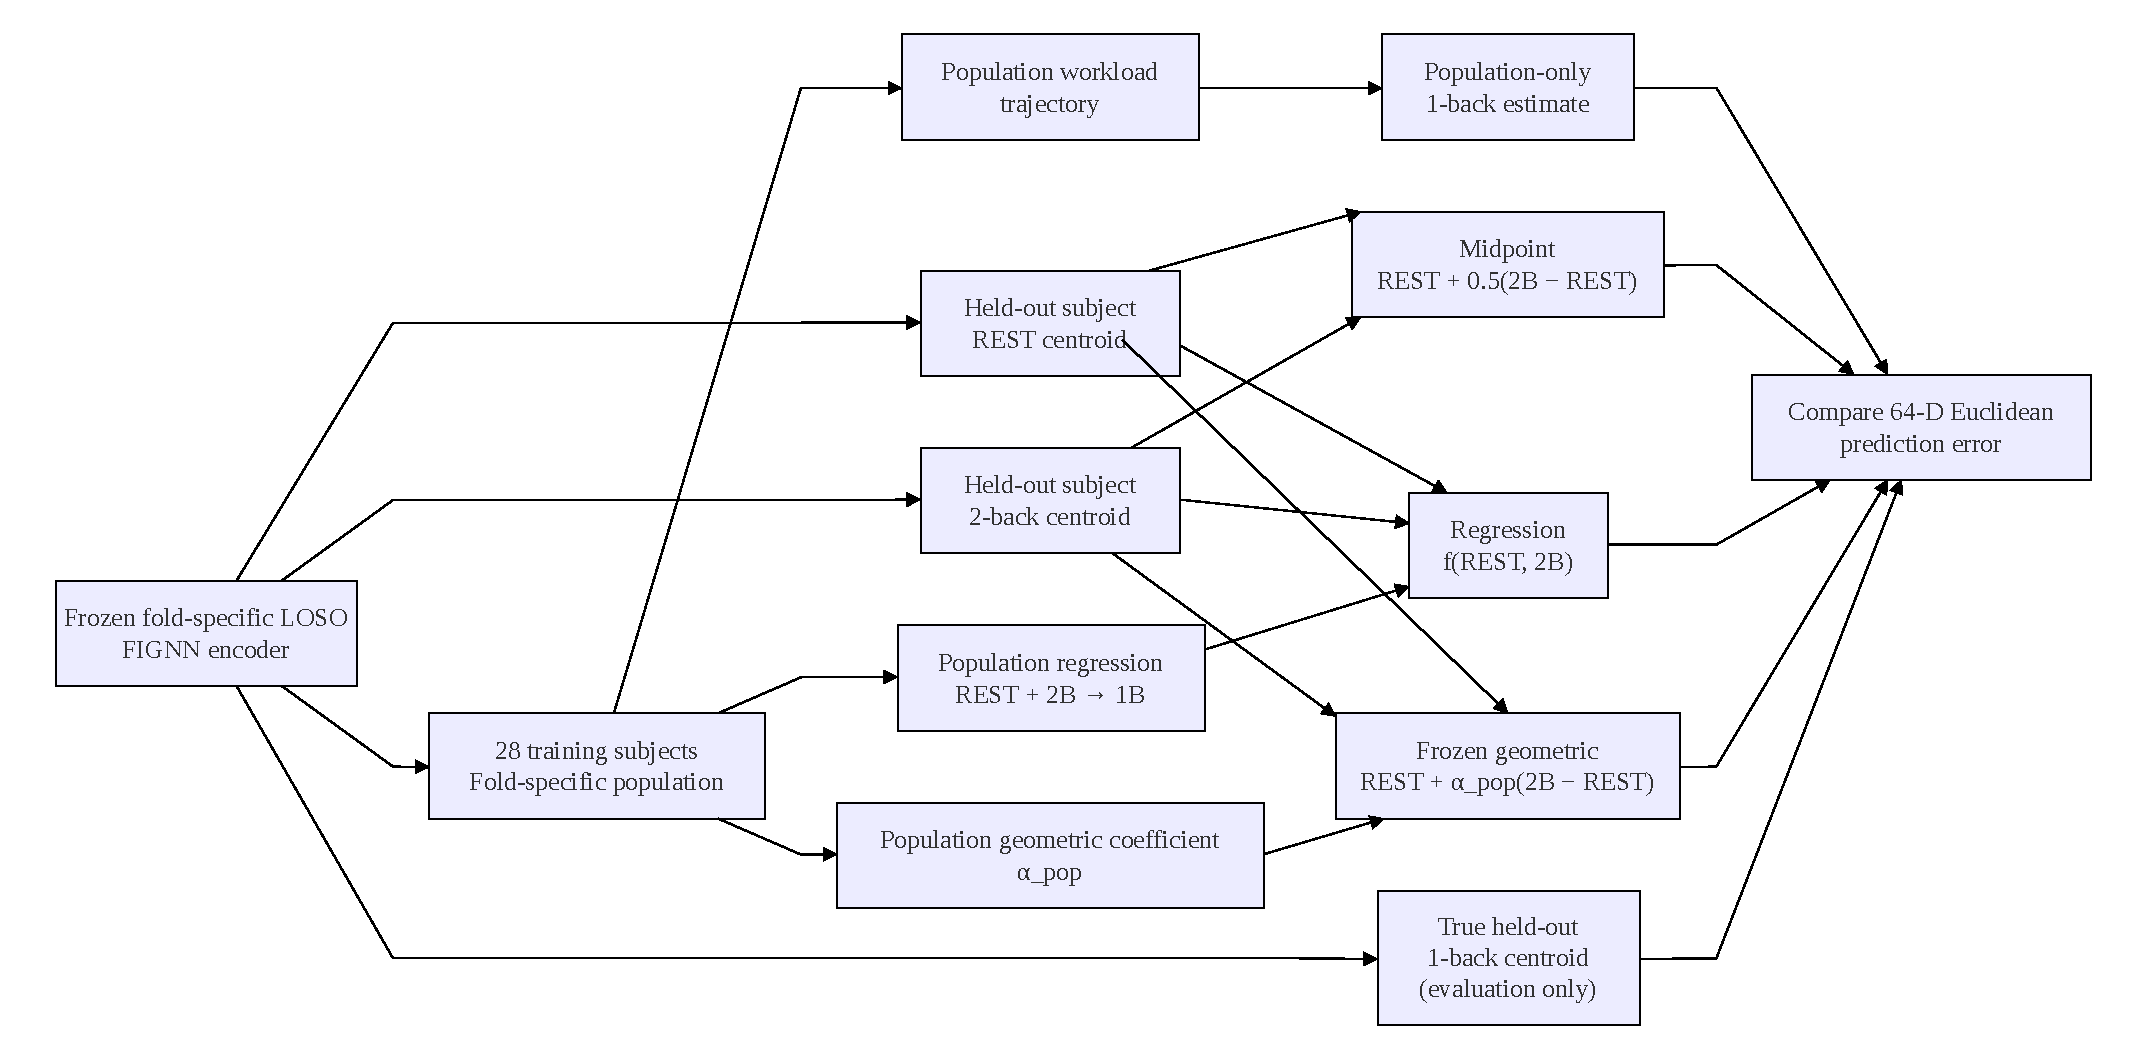
\includegraphics[width=0.92\textwidth]{figures/FIGNN_stage2_drawio.pdf}
\caption{Stage~2 frozen-encoder geometric calibration. The fold-specific
FIGNN encoder remains frozen throughout. Resting-state and known 2-back latent
anchors provide subject-specific reference points. Four methods are evaluated:
population-only (no subject data), midpoint (REST + 0.5$\cdot$(2B$-$REST)),
regression ($f$(\text{REST}, 2B)), and frozen geometric
($\alpha_{\mathrm{pop}}$ transferred onto the subject's REST-to-2-back
direction). The true held-out 1-back centroid is accessed only for evaluation.}
\label{fig:stage2_pipeline}
\end{figure*}

\subsection{Evaluation}

All four methods are evaluated against the true held-out 1-back centroid
using Euclidean distance in the full 64-dimensional latent space:
\begin{equation}
  \epsilon_s^{(\cdot)}
  = \bigl\|\widehat{\mathbf{C}}_{s,1}^{(\cdot)} - \mathbf{C}_{s,1}\bigr\|_2.
\end{equation}
Subject-level relative improvement over the population-only baseline is
\begin{equation}
  I_s = \frac{\epsilon_s^{\mathrm{pop}} - \epsilon_s^{(\cdot)}}
             {\epsilon_s^{\mathrm{pop}}} \times 100.
\end{equation}
Statistical comparisons against the population-only baseline use one-sided
paired Wilcoxon signed-rank tests (alternative: population-only error exceeds
method error) with Holm correction for multiple comparisons.

%% ============================================================
\section{Experimental Setup}
\label{sec:setup}
%% ============================================================

\subsection{Dataset}

The COG-BCI dataset contains EEG recordings from 29 participants across three
sessions and multiple cognitive tasks, including N-back, MATB, PVT, and Flanker
paradigms \cite{hinss2023}. The present study uses N-back recordings for the
graded workload trajectory analysis and resting-state (eyes-closed) recordings
for Stage~2 anchor computation. EEG was recorded at 500~Hz using a
64-electrode cap; participants~1--9 lack the Cz electrode, so the common
62-channel subset is used throughout.

The graph dataset contains 27\,666 total graphs across 29 subjects (954 per
subject). Of these, 25\,056 are N-back task graphs (864 per subject,
labels 0/1/2) used in Stage~1 training, and 2\,610 are REST graphs (90 per
subject, label~3) retained for Stage~2 anchor computation and excluded from
Stage~1.

\subsection{Preprocessing and Graph Construction}

EEG recordings are loaded from EEGLAB files using MNE-Python. Non-standard
channels are removed, a 50-Hz notch filter is applied, and average-reference
re-referencing is performed. Signals are separately band-pass filtered into
delta (1--4~Hz), theta (4--8~Hz), alpha (8--13~Hz), and beta (13--30~Hz).

N-back stimulus annotations are used to construct event-aligned epochs spanning
0--2~s from stimulus onset. Resting-state recordings are segmented into
non-overlapping 2-s windows. Relative band power is computed per retained
channel and within-band PLV is computed for all channel pairs. Edges are
retained when the mean four-band PLV exceeds 0.5.

\subsection{Evaluation Protocol}

All 29 subjects are evaluated individually under LOSO. For each fold,
normalization statistics are computed from the 28 training subjects' graphs and
applied to the held-out subject. The fold-specific checkpoint is frozen before
latent embeddings are generated.

Stage~1 conclusions are drawn primarily from the segment-membership criterion
$0\leq\rho_s\leq1$; $d_{01}<d_{02}$ serves as a supporting ordering diagnostic;
alignment-free trajectory metrics (path efficiency, $d_{01}/d_{02}$, angle)
provide descriptive characterization; and Procrustes similarity and direction
cosine are retained as secondary descriptive measures. Stage~2 compares four
methods; $\alpha_{\mathrm{pop}}$ and the regression model are fitted exclusively
from the 28 training subjects; the actual held-out 1-back centroid is used only
to compute evaluation error.

%% ============================================================
\section{Results}
\label{sec:results}
%% ============================================================

\subsection{Learned Band Importances}

After training across all 29 LOSO folds, the softmax-normalized frequency
weights $\mathbf{w}$ assigned the largest mean coefficients to the beta and
alpha bands. The mean values were $w_{\beta}=0.364$, $w_{\alpha}=0.291$,
$w_{\theta}=0.178$, and $w_{\delta}=0.168$. These coefficients characterize
the frequency weighting learned by FIGNN and should not be interpreted as
direct evidence of biological band dominance.

\subsection{Architecture Sensitivity}

To assess the sensitivity of the learned latent geometry to model capacity,
a 29-subject architecture comparison was conducted between the historical
64-hidden, 4-head, 32-dimensional latent configuration and the final
128-hidden, 8-head, 64-dimensional configuration, using the same corrected
subject-wise LOSO training protocol. Table~\ref{tab:arch} summarizes the
resulting trajectory geometry metrics. The two configurations produced
similar overall geometric behavior, with the final configuration yielding
$d_{01}/d_{02}=0.477$ compared with $0.587$ for the historical
configuration, and satisfying the supporting $d_{01}<d_{02}$ criterion in
27/29 versus 26/29 subjects. This comparison is treated as a sensitivity
analysis rather than a statistical superiority claim.

\begin{table}[!t]
  \caption{Architecture Sensitivity Across 29 Subjects}
  \label{tab:arch}
  \centering
  \begin{tabular}{lcc}
    \toprule
    \textbf{Metric} & \textbf{64/4/32} & \textbf{128/8/64 (final)} \\
    \midrule
    $d_{01}/d_{02}$        & 0.587 & 0.477 \\
    $d_{12}/d_{02}$        & 0.924 & 0.824 \\
    Path efficiency        & 0.771 & 0.819 \\
    Procrustes similarity  & 0.856 & 0.878 \\
    $d_{01}<d_{02}$        & 26/29 & 27/29 \\
    \bottomrule
  \end{tabular}
\end{table}

\subsection{Component Ablation}

Table~\ref{tab:ablation} presents a controlled four-fold component ablation
over held-out subjects~7, 15, 22, and~29. Seven variants are evaluated:
the full FIGNN model, and six ablated configurations removing or replacing
one component at a time. These results are intended as controlled sensitivity
evidence; because only four held-out subjects were used, no statistical
superiority claims are made.

\begin{table*}[!t]
  \caption{Controlled Four-Fold Component Ablation (Subjects 7, 15, 22, 29).
           All metrics are means over the four folds.
           GCN denotes the variant where GAT is replaced by GCN.}
  \label{tab:ablation}
  \centering
  \begin{tabular}{lccccr}
    \toprule
    \textbf{Variant}
      & $\mathbf{d_{01}/d_{02}}$
      & \textbf{Path efficiency}
      & \textbf{Procrustes}
      & \textbf{Dir.\ cosine}
      & \textbf{1B-between} \\
    \midrule
    Full FIGNN             & 0.398 & 0.833 & 0.784 & 0.919 & 3/4 \\
    No PLV                 & 0.527 & 0.821 & 0.742 & 0.931 & 3/4 \\
    No band weighting      & 0.459 & 0.801 & 0.744 & 0.927 & 2/4 \\
    Node-feature MLP       & 0.702 & 0.760 & 0.766 & 0.556 & 3/4 \\
    GCN replacing GAT      & 0.614 & 0.773 & 0.762 & 0.391 & 3/4 \\
    No SupCon              & 0.549 & 0.757 & 0.796 & 0.716 & 4/4 \\
    Band-power baseline    & 0.853 & 0.726 & 0.638 & 0.369 & 2/4 \\
    \bottomrule
  \end{tabular}
\end{table*}

Compared with the full model, removing PLV edges, removing learnable band
weighting, and replacing the band-power representation with a simpler baseline
all degrade one or more trajectory geometry metrics. Replacing GAT with GCN
notably reduces direction cosine, suggesting that edge-aware attention
contributes to trajectory orientation consistency. The ``No SupCon'' variant
achieves 4/4 on segment membership in this four-fold comparison, but shows
reduced path efficiency and direction cosine, consistent with less
well-organized overall trajectory geometry.

\subsection{PLV Threshold Sensitivity}

Table~\ref{tab:threshold} summarizes a frozen-model PLV-threshold sensitivity
analysis across thresholds $\{0.3, 0.4, 0.5, 0.6, 0.7\}$. At each threshold,
the graph topology is reconstructed from the cached per-band PLV records, while
the same fold-specific trained checkpoints and normalization statistics are used
without retraining. The primary criterion (1B-between) is stable at 23/29 for
thresholds 0.4--0.6 and reaches 25/29 at 0.7; path efficiency and Procrustes
similarity show modest variation across the range. These results indicate
broadly stable trajectory geometry under the frozen model across the tested
thresholds; they do not constitute threshold optimization.

\begin{table}[!t]
  \caption{Frozen-Model PLV Threshold Sensitivity (29 Subjects).
           No retraining is performed at any threshold.}
  \label{tab:threshold}
  \centering
  \begin{tabular}{ccccc}
    \toprule
    \textbf{Threshold}
      & \textbf{1B-between}
      & $\mathbf{d_{01}/d_{02}}$
      & \textbf{Path eff.}
      & \textbf{Procrustes} \\
    \midrule
    0.3 & 21/29 (72.4\%) & 0.628 & 0.767 & 0.807 \\
    0.4 & 23/29 (79.3\%) & 0.536 & 0.804 & 0.847 \\
    0.5 & 23/29 (79.3\%) & 0.477 & 0.819 & 0.878 \\
    0.6 & 23/29 (79.3\%) & 0.478 & 0.800 & 0.879 \\
    0.7 & 25/29 (86.2\%) & 0.549 & 0.788 & 0.850 \\
    \bottomrule
  \end{tabular}
\end{table}

\subsection{Stage 1: Cross-Subject Representation Transfer}

All 29 subjects were evaluated under strict LOSO using fold-specific frozen
checkpoints. The primary segment-membership criterion ($0\leq\rho_s\leq1$,
Equation~\ref{eq:rho}) is satisfied by \textbf{23 of 29} held-out subjects
(79.31\%; exact binomial 95\% CI: 60.3--92.0\%; one-sided exact test against
$p=0.5$: $p=0.0012$). The supporting distance-ordering criterion $d_{01}<d_{02}$
holds for 27 of 29 subjects (93.10\%).

Table~\ref{tab:stage1} reports the full set of alignment-free and secondary
descriptive metrics. Fig.~\ref{fig:trajectory_geom} shows the primary
Stage~1 trajectory geometry visualization, including the segment-membership
criterion and per-subject relative position values.

\begin{table}[!t]
  \caption{Stage~1 Trajectory Metrics Across 29 Held-Out Subjects (Mean $\pm$ SD)}
  \label{tab:stage1}
  \centering
  \begin{tabular}{lr}
    \toprule
    \textbf{Metric} & \textbf{Mean $\pm$ SD} \\
    \midrule
    \multicolumn{2}{l}{\emph{Primary}} \\
    Segment membership $0{\leq}\rho_s{\leq}1$ & 23/29 = 79.31\% \\
    \midrule
    \multicolumn{2}{l}{\emph{Supporting}} \\
    $d_{01}<d_{02}$                   & 27/29 = 93.10\% \\
    \midrule
    \multicolumn{2}{l}{\emph{Alignment-free descriptive}} \\
    Relative 1-back position $\rho_s$ & $0.271 \pm 0.291$ \\
    Perpendicular distance $\delta_s$ & $0.0135 \pm 0.0088$ \\
    $d_{01}/d_{02}$                   & $0.477 \pm 0.270$ \\
    $d_{12}/d_{02}$                   & $0.824 \pm 0.284$ \\
    Trajectory angle $\psi_s$ (deg)   & $73.2 \pm 39.7$ \\
    Path efficiency $\eta_s$          & $0.819 \pm 0.170$ \\
    Centrality                        & $0.421 \pm 0.457$ \\
    \midrule
    \multicolumn{2}{l}{\emph{Secondary descriptive}} \\
    Procrustes similarity $S_{\mathrm{proc}}$
                                      & $0.878 \pm 0.155$ \\
    Direction cosine $\cos\theta$     & $0.785 \pm 0.404$ \\
    \bottomrule
  \end{tabular}
\end{table}

\begin{figure}[!t]
\centering
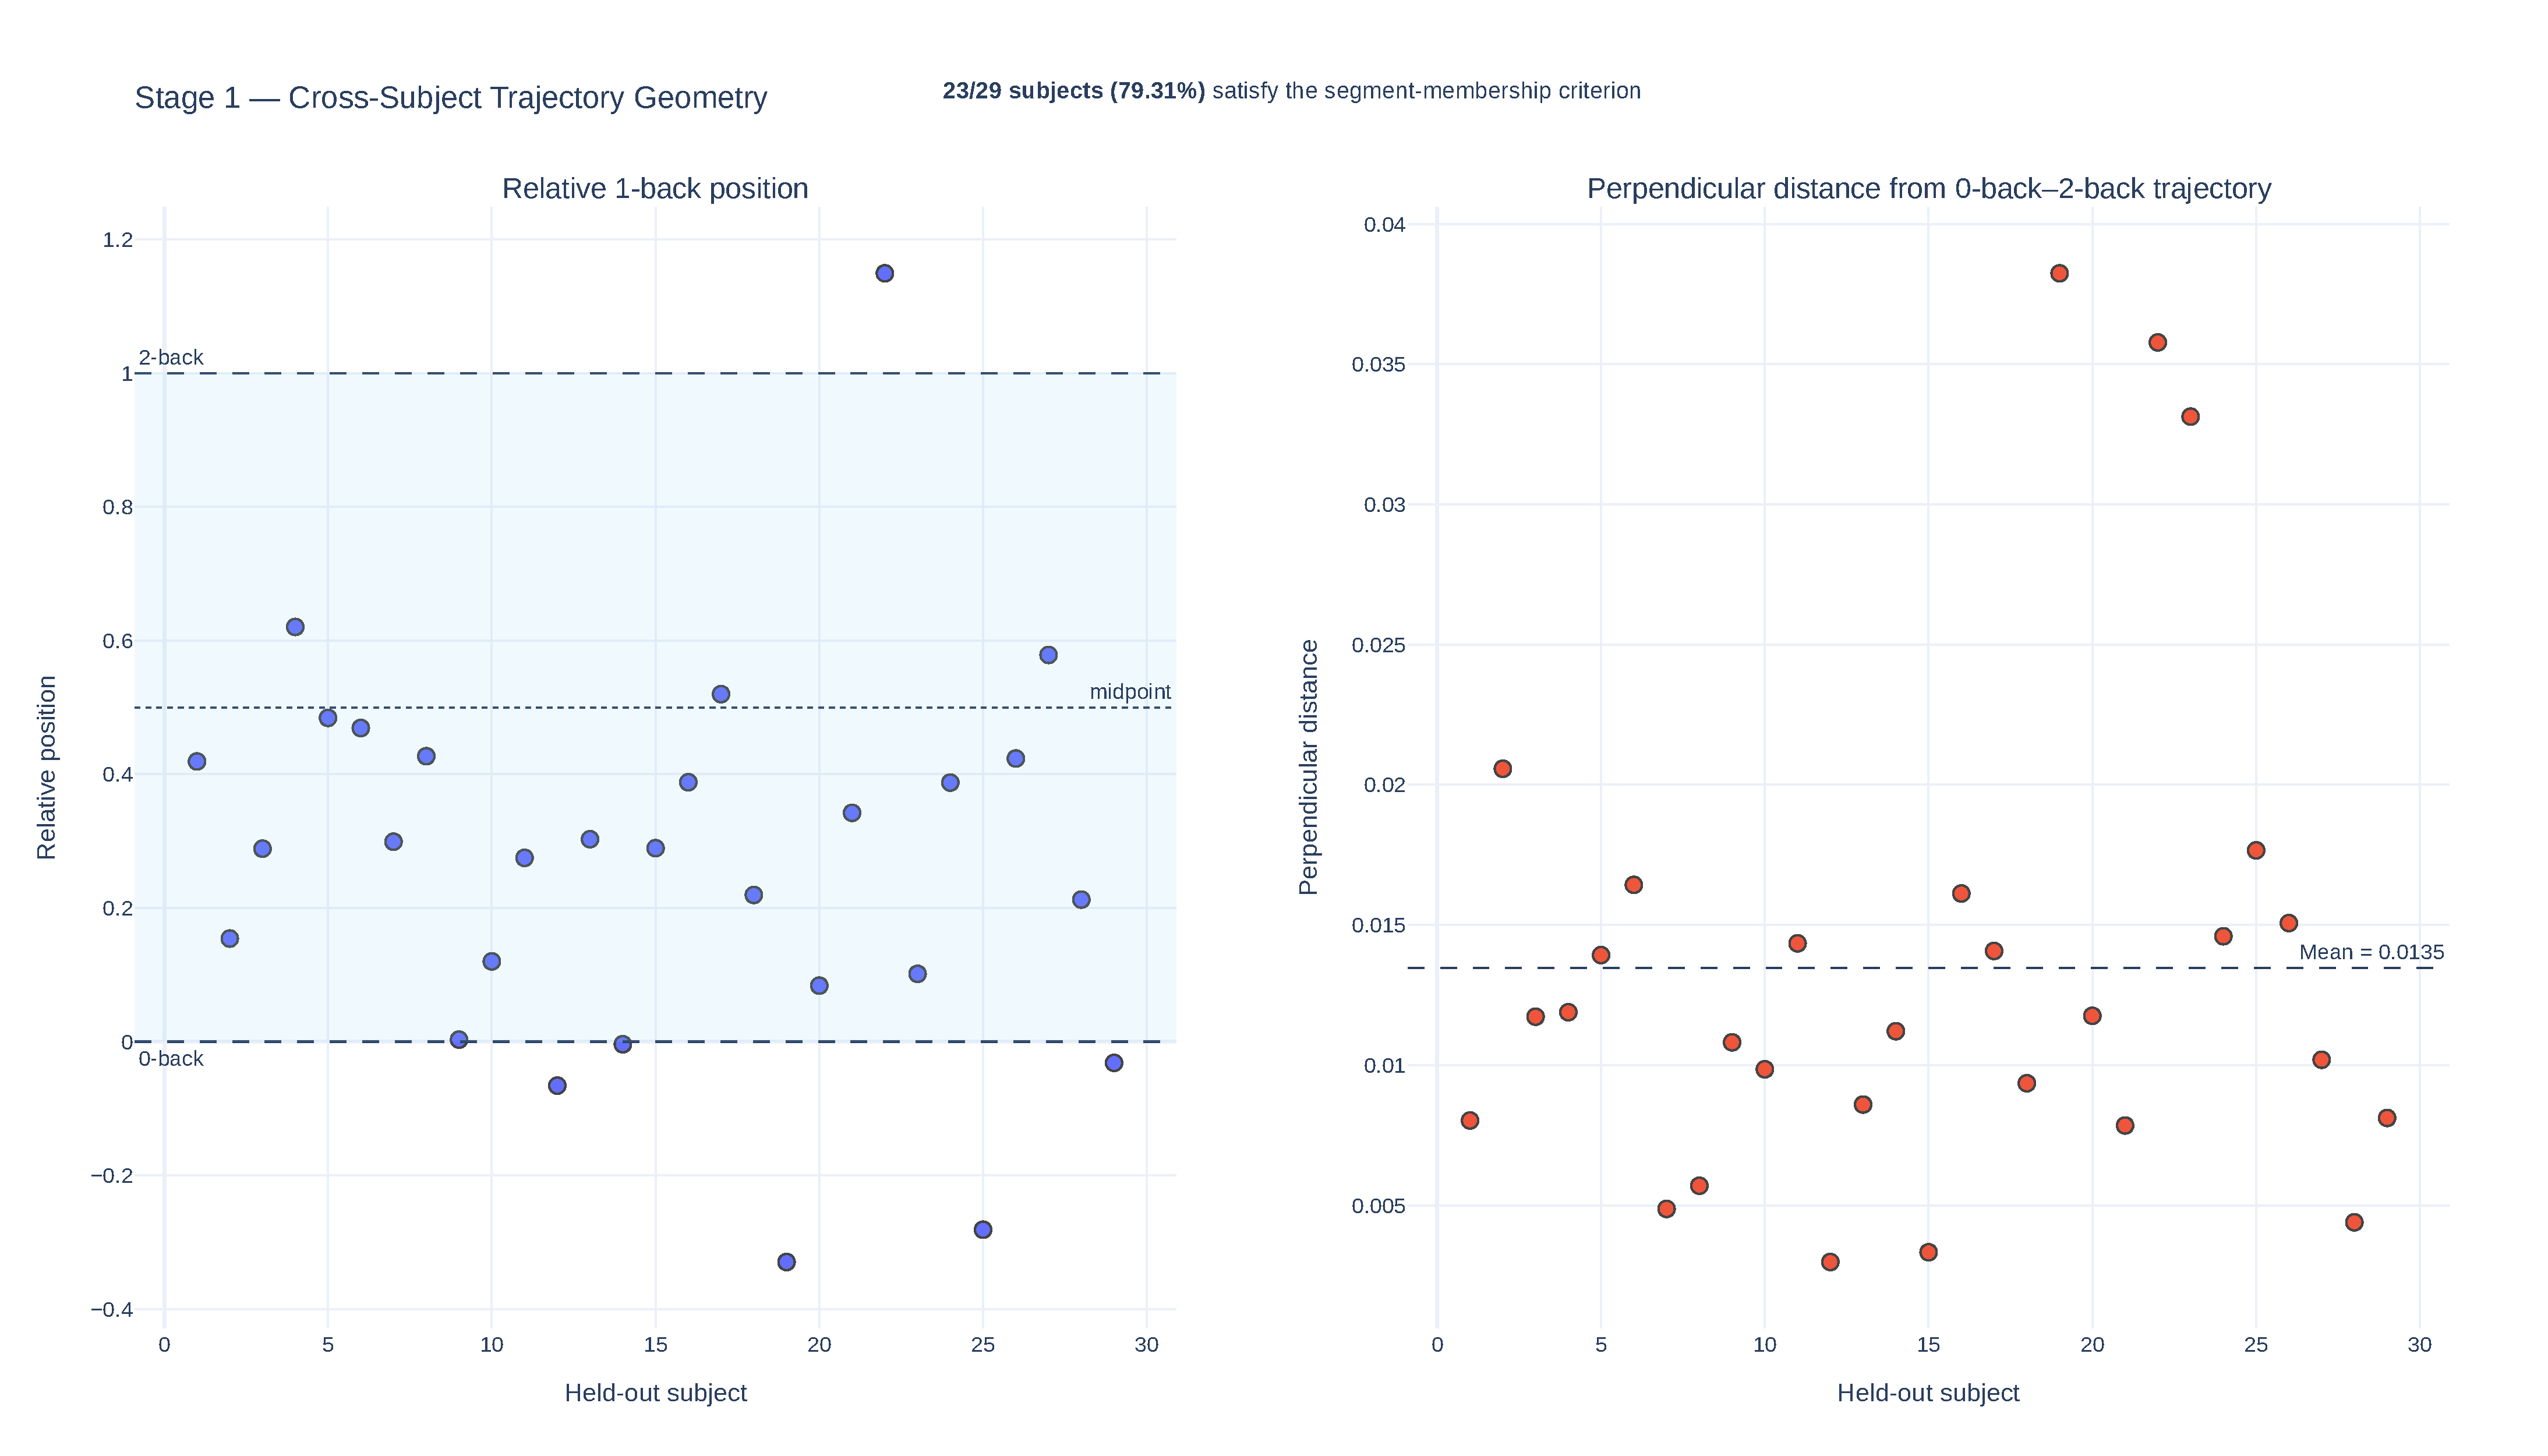
\includegraphics[width=\columnwidth]{figures/stage1_trajectory_geometry.pdf}
\caption{Stage~1 trajectory geometry across all 29 held-out subjects. The
figure shows the segment-membership criterion ($0\leq\rho_s\leq1$) and
per-subject relative 1-back position $\rho_s$, perpendicular distance
$\delta_s$, and path efficiency $\eta_s$. This is the primary Stage~1
visualization. All metrics are computed in the original 64-dimensional latent
space without alignment.}
\label{fig:trajectory_geom}
\end{figure}

The mean Procrustes similarity is $0.878\pm0.155$, retained as a secondary
descriptive measure. Because it is based on only three centroids in 64
dimensions, it is not treated as primary transferability evidence. The
Monte Carlo label-permutation null analysis found that 0 of 29 subjects
reached empirical $p<.05$, and the median observed Procrustes similarity
fell at approximately the 82.7th percentile of the subject-level null
distributions. This indicates that while the observed similarities are
generally above the null distribution mode, the three-point Procrustes
measure alone is not sufficient to rule out random alignment. The
alignment-free trajectory metrics and the binomial segment-membership result
provide the primary evidence.

The six subjects who fail the segment-membership criterion reflect genuine
inter-subject variability; their 1-back centroids lie outside the
0-back-to-2-back segment in the learned latent space. No specific
explanation is inferred for individual failures.

\subsubsection{Representative Unseen-Subject Trajectory}

Fig.~\ref{fig:subject17} provides a visualization for held-out subject~17.
Population and subject trajectories are aligned in the full 64-dimensional
space; the two-dimensional PCA projection is used only for illustration.
This figure is descriptive and representative only; subject~17 is not
statistically representative of the full cohort.

\begin{figure}[!t]
\centering
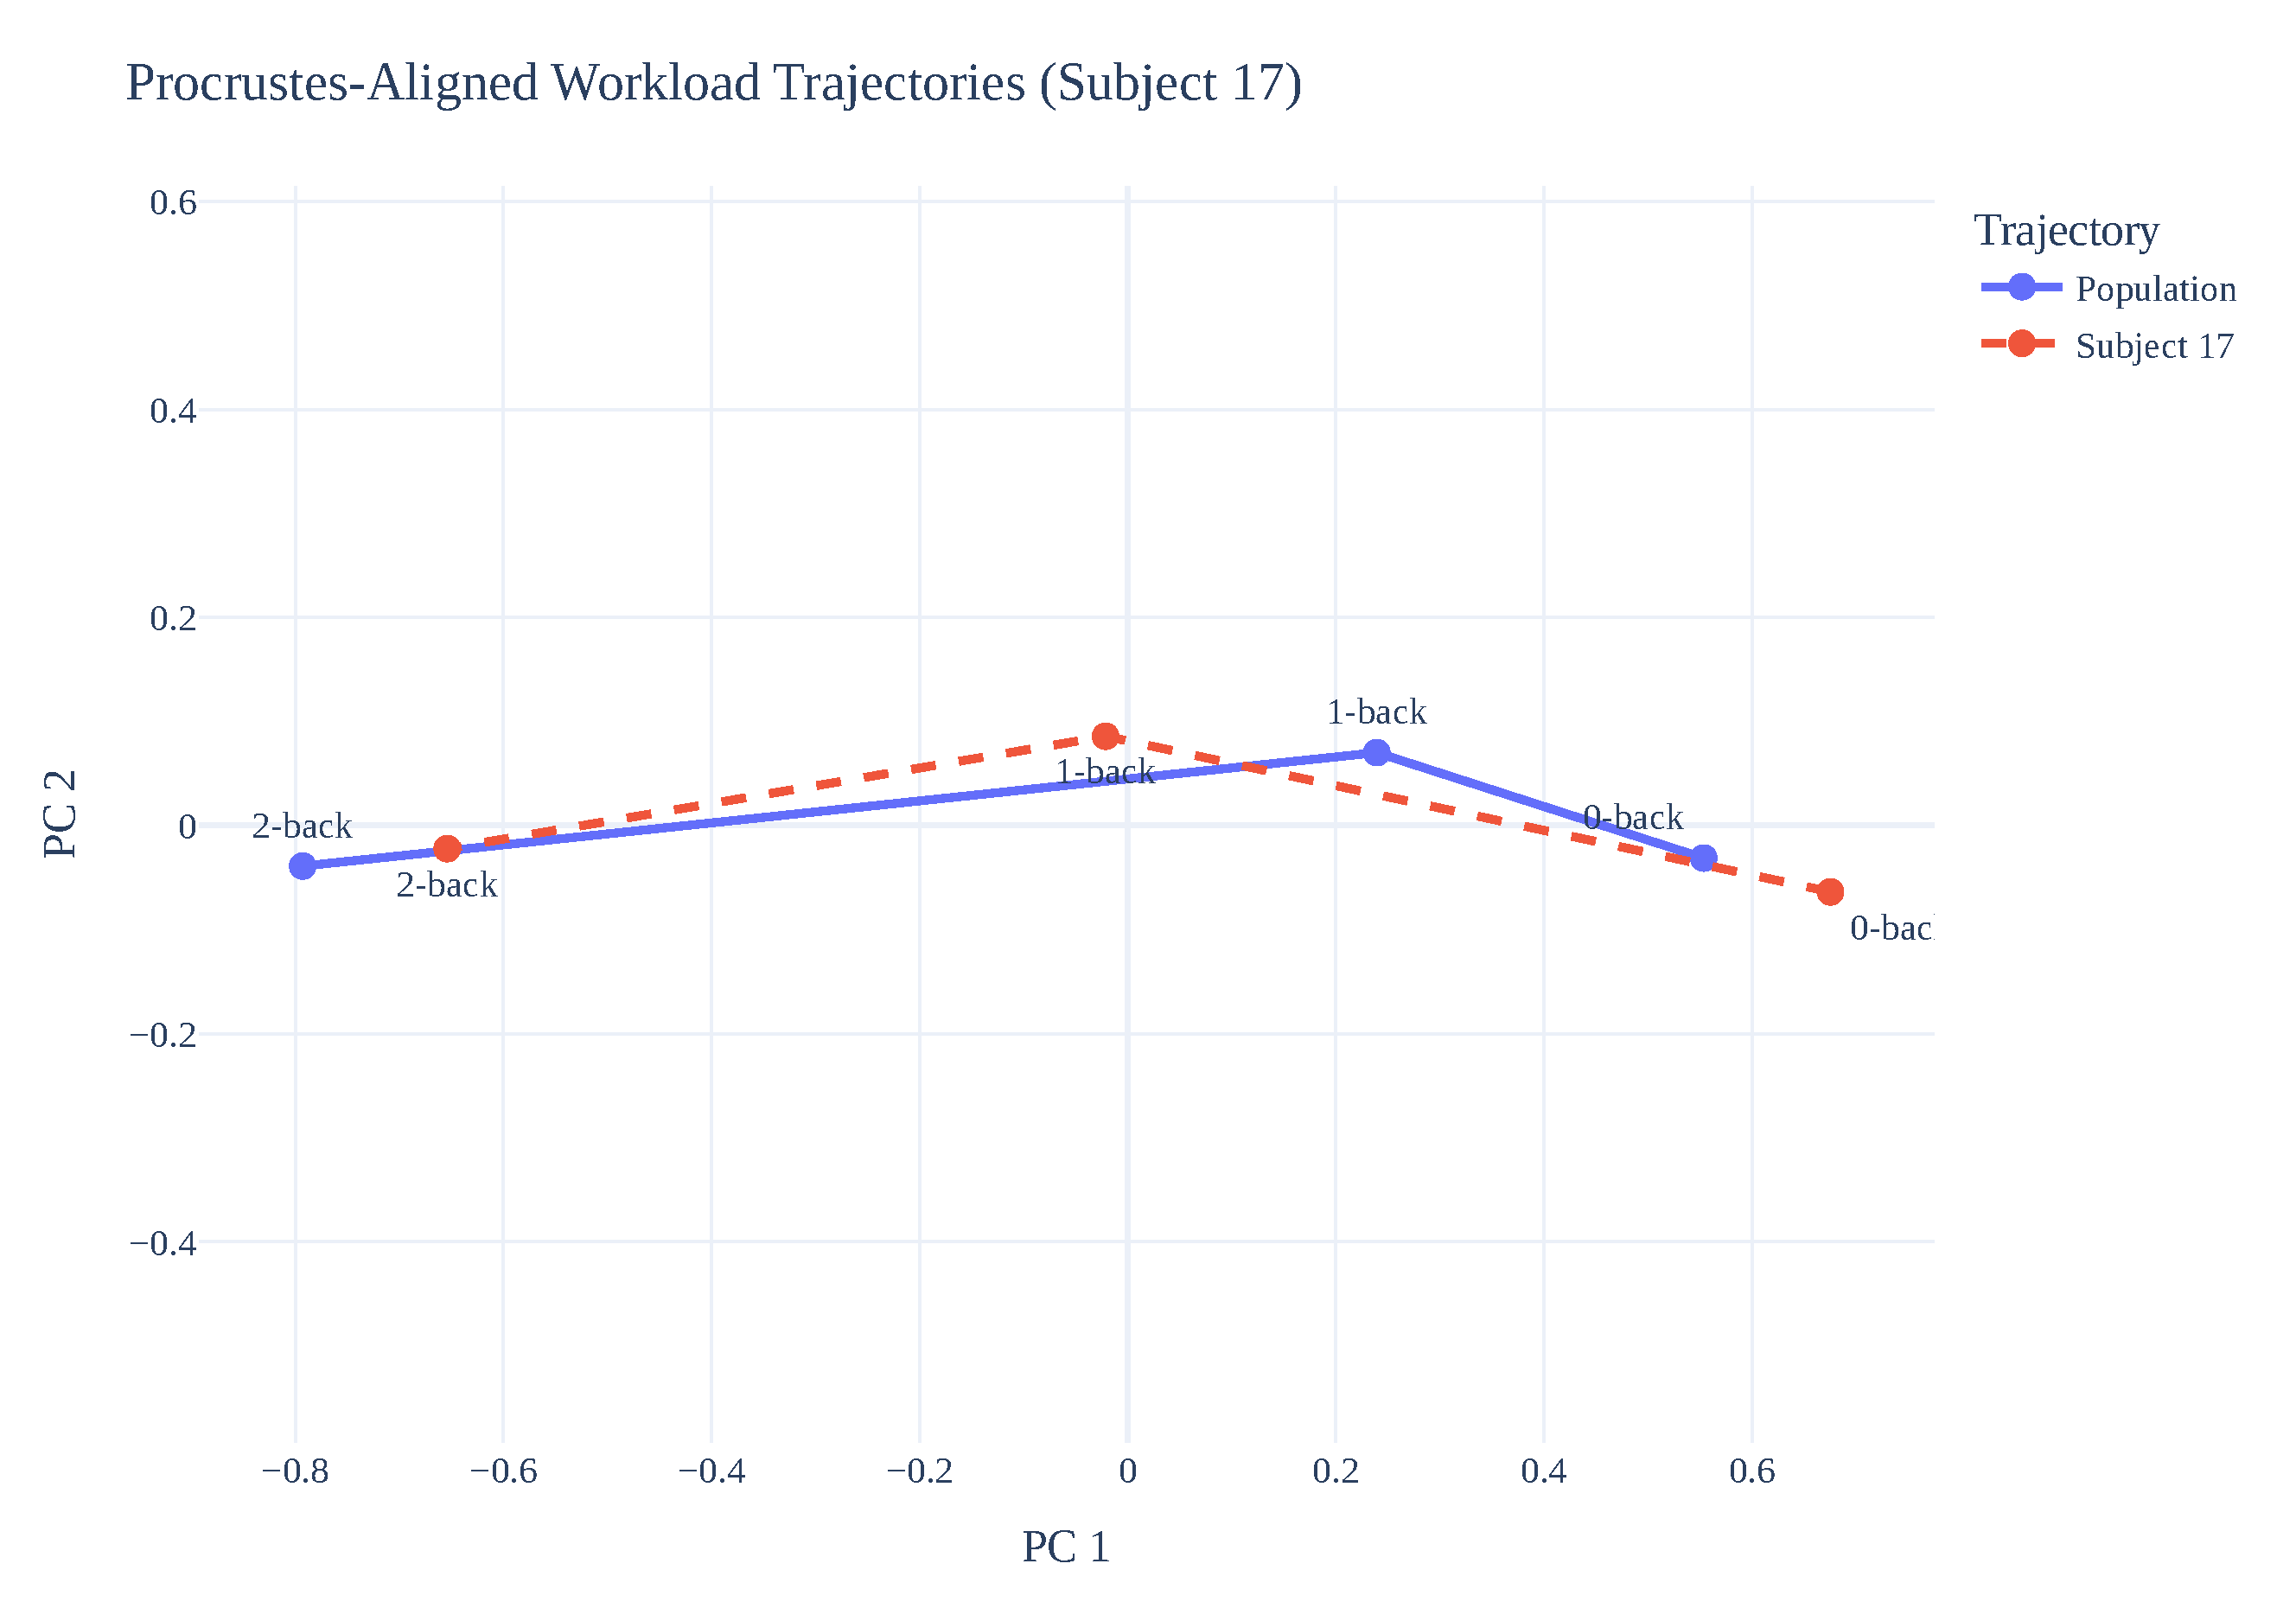
\includegraphics[width=\columnwidth]{figures/fig_procrustes_subject17.pdf}
\caption{Procrustes-aligned workload trajectories for representative
held-out subject~17. Population and subject trajectories are shown in a joint
two-dimensional PCA projection after alignment in the original 64-dimensional
latent space. This is a descriptive, qualitative illustration only.}
\label{fig:subject17}
\end{figure}

\subsubsection{REST Anchor Validation}

Because Stage~2 uses resting-state activity as a subject-specific reference,
the latent position of REST relative to the N-back workload states was first
assessed for all 29 held-out subjects. The mean Euclidean distances from the
REST centroid to the 0-back, 1-back, and 2-back centroids in the original
64-dimensional latent space were 0.1136, 0.1245, and 0.1561, respectively.
The monotonically increasing distance from REST toward higher workload states
provides descriptive supporting evidence that REST occupies a distinct
geometric reference position relative to the N-back states. REST is not
claimed to be completely separated from the 0-back cluster, and this
analysis does not constitute a formal cluster separation test.
Fig.~\ref{fig:rest} shows the per-subject REST-to-N-back distances.

\begin{figure}[!t]
\centering
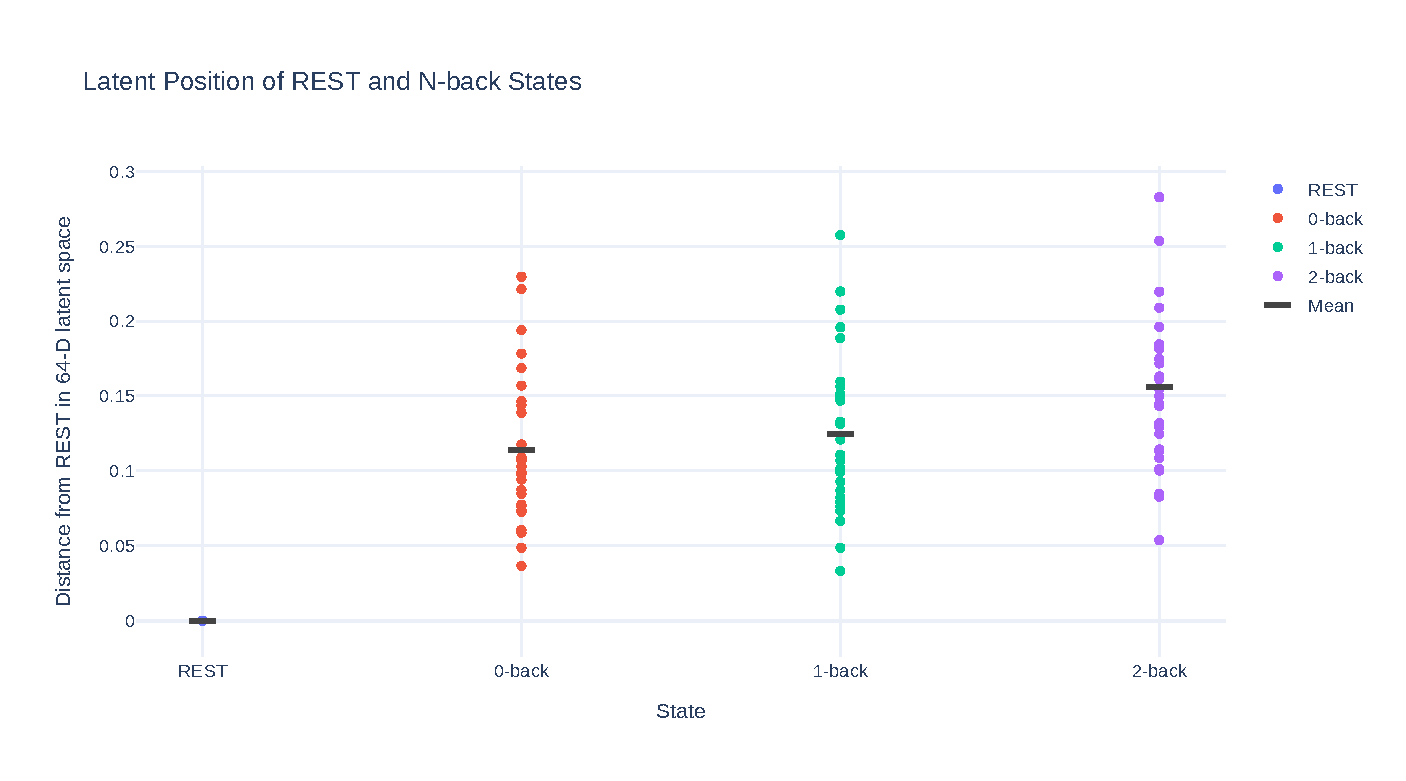
\includegraphics[width=\columnwidth]{figures/rest_nback_latent_distances.pdf}
\caption{REST-to-N-back latent distances across 29 held-out subjects. Each
dot shows the 64-dimensional Euclidean distance from a subject's REST centroid
to the 0-back, 1-back, and 2-back centroids. The monotonically increasing mean
distance supports REST as a plausible geometric reference for Stage~2
calibration. All distances are computed in the original 64-dimensional latent
space.}
\label{fig:rest}
\end{figure}

\subsection{Stage 2: Frozen-Encoder Geometric Calibration}

Table~\ref{tab:stage2} summarizes the 64-dimensional estimation error for all
four calibration methods across the 29 held-out subjects.

\begin{table}[!t]
  \caption{Stage~2 64-D Estimation Error for the Unseen 1-Back Centroid
           (29 Subjects). Wilcoxon tests are one-sided against the
           population-only baseline with Holm correction.}
  \label{tab:stage2}
  \centering
  \begin{tabular}{lcccc}
    \toprule
    \textbf{Method}
      & \textbf{Mean}
      & \textbf{SD}
      & \textbf{Median}
      & \textbf{Holm $p$} \\
    \midrule
    Population-only   & 0.0649 & 0.0319 & 0.0570 & - \\
    Midpoint          & 0.0522 & 0.0255 & 0.0503 & 0.091 \\
    Regression        & 0.0511 & 0.0303 & 0.0469 & 0.023 \\
    Frozen geometric  & \textbf{0.0345} & \textbf{0.0168} & \textbf{0.0298}
                      & \textbf{0.000404} \\
    \bottomrule
  \end{tabular}
\end{table}

The frozen geometric method achieves the lowest mean error (0.0345) and reduces
mean error by 0.0303 relative to the population-only baseline, corresponding to
a relative reduction of 46.74\% ($W=377$, raw $p=0.000135$, Holm $p=0.000404$,
Cohen's $d_z=0.821$, improved in 22/29 subjects). The regression baseline
(Holm $p=0.023$) also achieves statistical improvement, but with higher mean
error than the frozen geometric method and with a severely under-determined
regression problem (128 inputs, 64 outputs, 28 training samples). The midpoint
method does not reach the Holm significance threshold ($p=0.091$). The
population-only method requires no subject-specific data and serves as the
zero-calibration reference.

Fig.~\ref{fig:stage2_error} shows the per-subject error distributions for all
four methods.

\begin{figure*}[!t]
\centering
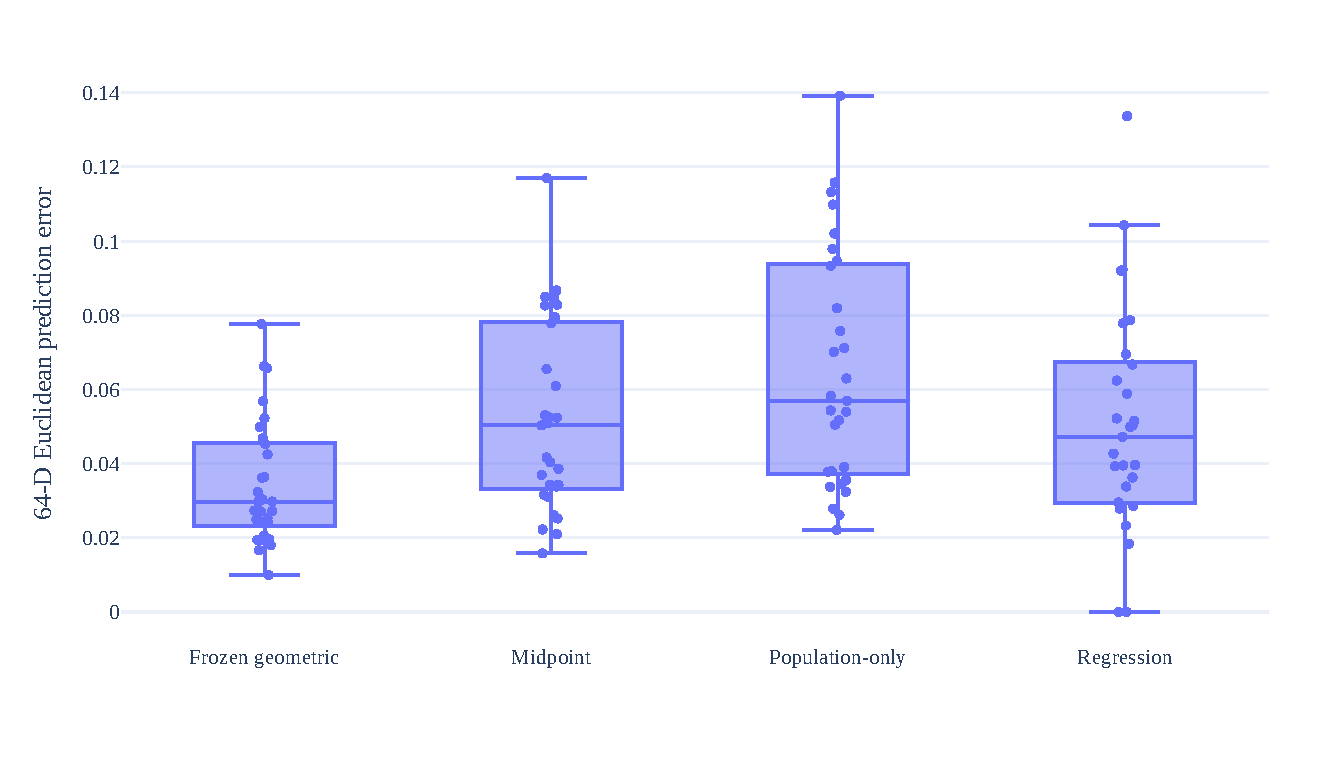
\includegraphics[width=0.92\textwidth]{figures/fig_stage2_calibration_error.pdf}
\caption{64-dimensional Euclidean estimation error for the unseen 1-back
centroid across the 29 held-out subjects (lower is better). All four
calibration methods are shown: population-only (no subject data),
midpoint, regression, and frozen geometric calibration using resting-state
and known 2-back anchors. The frozen geometric method achieves the lowest
error and is the only one to show both large effect size and Holm-corrected
significance relative to the population-only baseline.}
\label{fig:stage2_error}
\end{figure*}

%% ============================================================
\section{Discussion}
\label{sec:discussion}
%% ============================================================

\subsection{Geometric Transferability}

Within the COG-BCI dataset, the FIGNN representation demonstrates
evidence of cross-subject workload trajectory transfer. The primary
segment-membership criterion is satisfied by 23 of 29 held-out subjects;
six subjects fail, reflecting genuine inter-subject variability that the
current framework does not fully account for. The supporting distance-ordering
criterion ($d_{01}<d_{02}$) holds for 27 of 29 subjects, a weaker condition
that does not imply segment membership but corroborates the broad trend.

The observed workload trajectory ordering is an emergent geometric property of
the supervised contrastive representation rather than an ordering explicitly
imposed by the objective. The SupCon loss pulls same-label embeddings together
and separates different-label embeddings, but imposes no ordinal constraint
on the 0-back, 1-back, 2-back sequence. That 23 of 29 subjects show
segment-consistent geometry therefore provides evidence that the learned
representation structure is informative about relative workload across subjects.

The Procrustes similarity ($0.878\pm0.155$) is retained as a secondary
descriptive measure. Because it is based on only three centroids in a
64-dimensional space, it cannot independently establish transferability:
the Monte Carlo permutation analysis confirms that the observed values, while
generally above the null mode (median observed percentile $\approx82.7$th),
do not achieve per-subject statistical significance ($p<.05$) under label
permutation for any of the 29 subjects. Direction cosine provides an
additional orientation diagnostic but is not independent of Procrustes
analysis.

\subsection{Calibration Without Encoder Retraining}

Stage~2 demonstrates that transferable geometry and personalization are
complementary. The frozen geometric method reduces mean 64-dimensional
estimation error by 46.74\% relative to the population-only baseline, with
a large effect size ($d_z=0.821$) and Holm-corrected significance
($p=0.000404$). This reduction is achieved without any gradient-based
adaptation of the encoder - the fold-specific model parameters remain
entirely frozen.

The seven subjects for whom frozen geometric calibration does not improve
the estimate likely reflect cases where the subject's idiosyncratic REST-to-2-back
direction is less aligned with the population template, causing the transferred
$\alpha_{\mathrm{pop}}$ to misplace the intermediate state. Additional anchor
states or nonlinear placement strategies may be required for these subjects.

The regression baseline achieves Holm-corrected significance ($p=0.023$) but
with a substantially higher mean error than frozen geometric calibration and
an inherently under-determined mapping. The midpoint baseline does not achieve
significance, indicating that naive midpoint interpolation is insufficient.

\subsection{Limitations and Future Work}
\label{sec:limitations}

Several limitations constrain the current conclusions. First, the evaluation
uses only the COG-BCI dataset; generalization to other EEG datasets, recording
setups, and workload paradigms cannot be established from these results.
Second, the primary criterion is satisfied by 23/29, not all subjects;
inter-subject variability remains substantial. Third, Procrustes similarity
is based on only three workload centroids in a 64-dimensional space and is
reported as descriptive only. Fourth, the lower end of the delta band
(1--4~Hz) has a limited number of cycles within 2-s event-aligned epochs;
while such epoch lengths are used in PLV connectivity analyses in the
literature, the reliability of delta-band PLV at 2~s is a methodological
constraint. Fifth, the frozen-model PLV threshold sensitivity analysis does
not involve retraining and therefore does not identify the globally optimal
threshold; it characterizes sensitivity of the existing model to threshold
choice only. Sixth, Stage~2 still requires resting-state and known 2-back
measurements from each new subject, reducing but not eliminating subject-specific
data requirements. Seventh, the regression baseline in Stage~2 has an
under-determined feature dimensionality relative to training-sample count.
Eighth, the evaluation is focused on latent trajectory geometry rather than
continuous deployment-level workload prediction.

Future work can explore: (i)~additional anchor configurations and nonlinear
placement strategies for Stage~2; (ii)~alternative graph connectivity metrics
in conjunction with PLV; (iii)~extension to continuous workload trajectories
beyond discrete N-back levels; (iv)~external dataset validation; and
(v)~the quantum-inspired encoder extension as a comparative experiment on
the same LOSO protocol.

%% ============================================================
\section{Conclusion}
\label{sec:conclusion}
%% ============================================================

This paper presented FIGNN, a Frequency-Informed Graph Neural Network for
cross-subject EEG workload representation and frozen-encoder geometric
calibration. The model encodes EEG epochs as 62-channel graphs with relative
four-band power at the nodes and frequency-specific PLV at the edges. A
learnable frequency-weighting layer, which assigns the largest learned
coefficients to beta ($w=0.364$) and alpha ($w=0.291$), modulates edge
attributes before edge-aware graph attention produces a normalized 64-dimensional
embedding. The encoder is trained with supervised contrastive learning; the
observed workload trajectory ordering is an emergent geometric property of
the representation, not explicitly imposed by the contrastive objective.

Under strict 29-fold LOSO evaluation on the COG-BCI dataset, the primary
segment-membership criterion ($0\leq\rho_s\leq1$) is satisfied by 23 of 29
held-out subjects (79.31\%; exact binomial 95\% CI: 60.3--92.0\%;
$p=0.0012$ vs.\ chance). The supporting distance-ordering criterion
$d_{01}<d_{02}$ holds for 27 of 29 subjects. Mean alignment-free trajectory
metrics include path efficiency $0.819\pm0.170$ and $d_{01}/d_{02}$
$0.477\pm0.270$. The mean Procrustes similarity ($0.878\pm0.155$) is retained
as a secondary descriptive measure only; the permutation null analysis
confirms it cannot independently establish transferability.

A frozen-model PLV threshold sensitivity analysis (thresholds 0.3--0.7)
shows broadly stable primary criterion and trajectory metrics under the
existing checkpoints, without any retraining. A controlled four-fold component
ablation provides sensitivity evidence supporting the relevance of PLV
connectivity, learnable band weighting, edge-aware GAT, and the supervised
contrastive objective; results are from four held-out subjects and do not
support statistical superiority claims.

Stage~2 frozen-encoder geometric calibration reduces mean 64-dimensional
1-back estimation error from 0.0649 to 0.0345 (46.74\% relative reduction),
improving 22 of 29 subjects without any encoder retraining
($W=377$, Holm $p=0.000404$, Cohen $d_z=0.821$). These results, specific
to the COG-BCI dataset, support a population-to-personalization paradigm in
which a common latent workload geometry is transferred to an unseen subject
and subsequently adapted using minimal subject-specific information.

%% ============================================================
\section*{Acknowledgment}
%% ============================================================
The authors acknowledge the Centre for Neuroinformatics for providing the
research environment and support for this work. The authors also acknowledge
the COG-BCI dataset \cite{hinss2023}.

In accordance with IEEE policy, the authors disclose that ChatGPT (OpenAI)
was used to assist with manuscript drafting, language editing, and
organization. The scientific methodology, experimental implementation,
analysis, interpretation of results, and final manuscript content were
reviewed and verified by the authors.


\bibliographystyle{IEEEtran}
\bibliography{references}

\EOD
\end{document}